%
% vergleich.tex -- vergleich von signalen
%
% (c) 2019 Prof Dr Andreas Müller, Hochschule Rapperswil
%
\section{Vergleich von Signalen und Vektorgeometrie
\label{section:vergleich}}
\rhead{Vergleich von Signalen und Vektorgeometrie}
In diesem Abschnitt suchen wir eine geometrische Sprache für das
Problem, zwei Signale zu vergleichen und ein Signal aus geeigneten
Vergleichssignalen zusammenzusetzen.

\subsection{Vergleich von Signalen}
Beginnend mit Binärsignalen entwickeln wir ein anschauliches Mass für die
``Ähnlichkeit'' von zwei Signalen.

\subsubsection{Binärsignale}
Wir beginnen unsere Betrachtungen mit zwei diskrete Signale mit Werten $\pm 1$:
\[
\begin{aligned}
&x_1,x_2,x_3,\dots,x_N &&\in \{\pm 1\},
\\
&y_1,y_2,y_3,\dots,y_N &&\in \{\pm 1\}
\end{aligned}
\]
und versuchen eine Masszahl für die Ähnlichkeit dieser beiden
Zahlfolgen zu entwickeln.

Die Masszahl muss umso grösser sein, je öfter die Folgenglieder
übereinstimmen, also $x_k=y_k$.
Indizes $k$, für die die Folgenglieder entgegengesetzt sind, also
$x_k\ne y_k$, müssen dagegen abgezogen werden.
Eine mögliche Masszahl ist daher 
\[
\sum_{k=1}^N x_ky_k.
\]
Sind die beiden Folgen identisch, wird die Summe $N$.
Sind die beiden Folgen genau entgegengesetzt, also $x_k=-y_k$, dann ist
sie $-N$.
Die Masszahl ist damit abhängig von der Anzahl der Datenpunkte.
Damit wird es nicht gut möglich, Funktionsvergleiche über verschieden
lange Datensätze miteinander zu vergleichen.
Das Problem wird gelöst, indem man durch $N$ teilt und als Masszahl
\[
p=\frac{1}{N} \sum_{k=1}^N x_ky_k
\]
verwendet.
Die Extremwerte werden jetzt $p=1$ für übereinstimmende Signale und
$p=-1$ für entgegengesetzte Signale.

Wenn die beiden Folgen nichts mitenander zu tun haben, dann erwarten
wir, dass $x_k$ und $y_k$ jeweils etwa in der Hälfte der Fälle
entgegengesetztes Vorzeichen haben werden und gleiches in allen
anderen.
Dies führt auf $p=0$.
Die Zahl $p$ könnte also als Mass dafür dienen, wie ähnlich die beiden Signale
sind.

Dies ist allerdings nicht ganz realistisch.
Warum sollten die Werte $+1$ und $-1$ gleich häufig sein?
Man könnte dies korrigieren, indem man den mittleren Wert beider Folgen
subtrahiert.
So erhält man die Kovarianz
\index{Kovarianz}%
\begin{equation}
\operatorname{cov}(x_k,y_k)
=
\frac1{N} \sum_{k=1}^N x_ky_k
-
\frac1{N} \sum_{k=1}^N x_k
\cdot
\frac1{N} \sum_{k=1}^N y_k.
\label{geometrie:cov}
\end{equation}
Die Kovarianz verschwindet genau dann, wenn beiden Signale $x_k$ und $y_k$
völlig unkorreliert sind.
Offenbar reicht es auch vollständig aus, wenn nur eines der Signale
im Mittel den Wert $0$ hat, dann verschwindet der zweite Term
in~\eqref{geometrie:cov}.

\subsubsection{Reellwertige Signale}
\begin{figure}
\centering
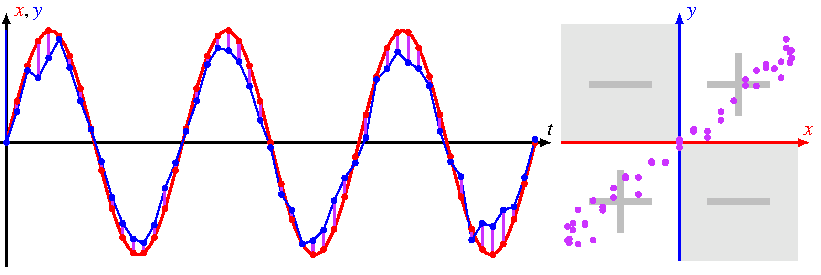
\includegraphics[width=\hsize]{chapters/1-geometrie/images/sinsin.pdf}
\caption{Vergleich eines Sinus-Signals $\color{red}x(t)$ mit einem
verrauschten Sinus-Signal $\color{blue}y(t)$.
Die Punkte $({\color{red}x(t)},{\color{blue}y(t)})$ befinden sich
hauptsächlich im ersten und dritten Quadranten.
\label{geometrie:kovarianz:sinsin:image}}
\end{figure}
\begin{figure}
\centering
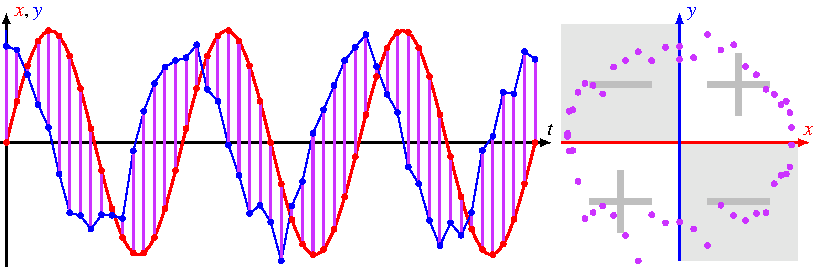
\includegraphics[width=\hsize]{chapters/1-geometrie/images/sincos.pdf}
\caption{Vergleich eines Sinus-Signals $\color{red}x(t)$ mit einem
verrauschten Kosinus-Signal $\color{blue}y(t)$.
Die Punkte $({\color{red}x(t)},{\color{blue}y(t)})$ befinden sich
in ungefähr gleicher Zahl in allen vier Quadranten, die Kovarianz
wird klein sein.
\label{geometrie:kovarianz:sincos:image}}
\end{figure}
\begin{figure}
\centering
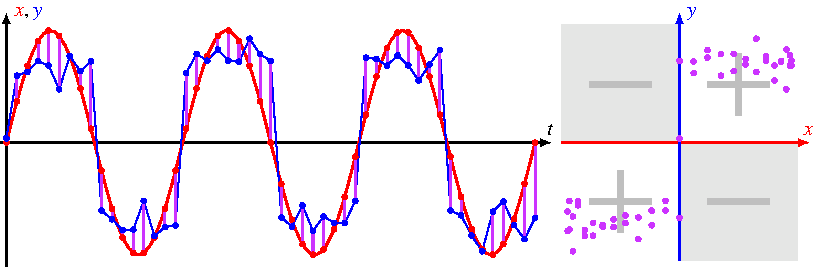
\includegraphics[width=\hsize]{chapters/1-geometrie/images/sinrect.pdf}
\caption{Vergleich eines Sinus-Signals $\color{red}x(t)$ mit einem
verrauschten Rechteck-Signal $\color{blue}y(t)$.
Die Punkte $({\color{red}x(t)},{\color{blue}y(t)})$ befinden sich
hauptsächlich im ersten und dritten Quadranten.
\label{geometrie:kovarianz:sinrect:image}}
\end{figure}
\begin{figure}
\centering
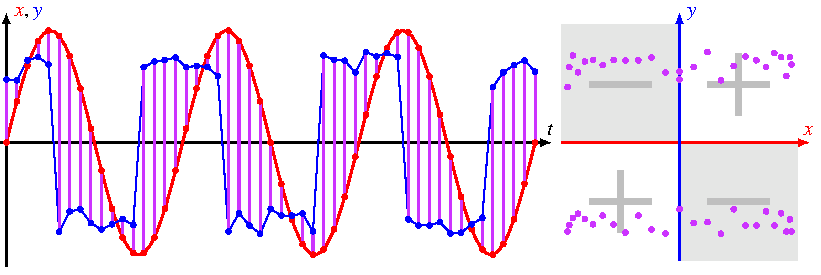
\includegraphics[width=\hsize]{chapters/1-geometrie/images/cosrect.pdf}
\caption{Vergleich eines Sinus-Signals $\color{red}x(t)$ mit einem
verrauschten und phasenverschobenen Rechteck-Signal $\color{blue}y(t)$.
Die Punkte $({\color{red}x(t)},{\color{blue}y(t)})$ befinden sich
in ungefähr gleicher Zahl in allen vier Quadranten, die Kovarianz
wird klein sein.
\label{geometrie:kovarianz:cosrect:image}}
\end{figure}
\begin{figure}
\centering
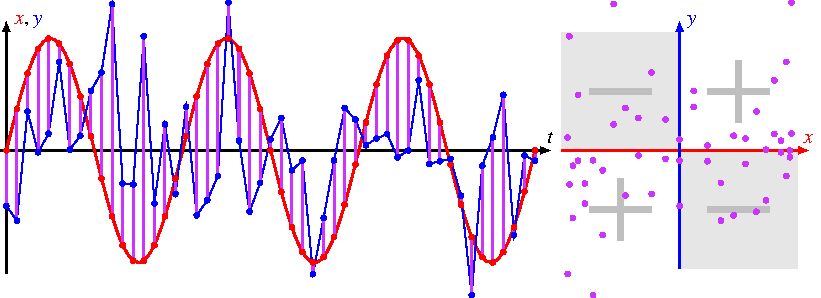
\includegraphics[width=\hsize]{chapters/1-geometrie/images/sinrand.pdf}
\caption{Vergleich eines Sinus-Signals $\color{red}x(t)$ mit einem
weissen Rausch-Signal $\color{blue}y(t)$ (normalverteilte Zufallswerte
mit Erwartungswert $0$).
Die Punkte $({\color{red}x(t)},{\color{blue}y(t)})$ befinden sich
in ungefähr gleicher Zahl in allen vier Quadranten, die Kovarianz
wird klein sein.
\label{geometrie:kovarianz:sinrand:image}}
\end{figure}


Binäre Signale sind nicht allgemein genug, wir möchten daher zwei
beliebige rellwertige Signale vergleichen.
Die früher verwendete Summe der Produkte der Signalwerte wird grösser,
wenn die Signalwerte grösser werden, sie ist also nicht geeignet als
absolutes Mass für die Ähnlichkeit zweier Funktionen.
Wir müssen daher mit einem Faktor korrigieren, der die ungefähre
Grösse der Absolutbeträge des Signals wiedergibt.
Der Mittelwert ist dazu nicht geeignet, da er bei Werten mit verschiedenen
Vorzeichen verschwinden kann.
Der Absolutbetrag ist eine nicht differenzierbare Funktion und damit
oft etwas unhandlich.
Es drängt sich daher auf, die quadratischen Mittelwerte
\[
\frac1{N}
\sum_{k=1}^N x_k^2
\qquad\text{bzw.}\qquad
\frac1{N}
\sum_{k=1}^N y_k^2
\]
zu
verwenden.
Diese haben allerdings die falsche Masseinheit, nämlich die des
Quadrates des Signals, wir müssen also ihre Quadratwurzel verwenden.
Für Signale mit Mittelwert $0$ führt dies auf
\[
\frac{
\frac{1}{N}\sum_{k=1}^N x_ky_k
}{
\sqrt{\frac{1}{N}\sum_{k=1}^N x_k^2}
\sqrt{\frac{1}{N}\sum_{k=1}^N y_k^2}
}
\qquad\text{oder}\qquad
r
=
\frac{\operatorname{cov}(x_k,y_k)}{\sqrt{\mathstrut\operatorname{var}(x_k)}\sqrt{\mathstrut\operatorname{var}(y_k)}}
\]
Die Grösse $r$ ist auch bekannt als der Korrelationskoeffizient.
\index{Korrelationskoeffizient}%
\index{Varianz}%

\subsubsection{Beispiele}
Wir illustrieren die eben entwickelten Konzepte an Hand einiger Beispiele
in den Abbildungen~\ref{geometrie:kovarianz:sinsin:image} bis
\ref{geometrie:kovarianz:sinrand:image}.

In den Abbildung~\ref{geometrie:kovarianz:sinsin:image} bis
\ref{geometrie:kovarianz:sinrand:image} wird ein Sinus-Signal
mit Werten $x(t)=\sin t$ abgetastet und verglichen mit
einer Reihen anderer Signale,
die alle ebenfalls den Mittelwert $0$ haben.
Wir wollen beurteilen, wie gut die Summe
\[
\frac{1}{N}\sum_{k=1}^N x_ky_k
\]
wiedergibt, ob die Funktionen etwas miteinander zu tun haben.
Dazu wird im linken Teil der Abbildung jeweils das Sinus-Signal
$x(t)$ rot eingezeichnet und das damit zu vergleichende Signal $y(t)$
blau.
Der Unterschiede zwischen den beiden Werten wird durch einen 
violetten Balken eingezeichnet.

Im rechten Teil der Abbildung wird dann für jeden Zeitpunkt
das Wertepaar $(x(t),y(t))$ als violetter Punkt eingetragen.
Punkte im ersten und dritten Quadranten führen auf einen positiven
Summanden in der Summe, Punkte im zweiten und vierten Quadranten
führen auf einen negativen Beitrag.
Die Summe wird also besonders gross, wenn die violetten Punkte vor
Allem im ersten und dritten Quadranten liegen, und besonders negativ,
wenn sie vor Allem im zweiten und vierten Quadranten liegen.

Liegen die violetten Punkte ungefähr gleich häufig in allen vier Quadranten,
ist davon auszugehen, dass sich die positiven und negativen Werte des
Produktes im Mittel wegheben werden, dass also die Summe der
Produkte nur einen kleinen Wert haben wird.

Die Abbildungen~\ref{geometrie:kovarianz:sinsin:image} und
\ref{geometrie:kovarianz:sinrect:image} zeigen den Vergleich
des Sinus-Signals mit einer verrauschten Version eines Sinus-Signals
bzw.~eines Rechteck-Signals $\operatorname{sign}(\sin(t))$.
In beiden Fällen liegen die violetten Punkte vorzugsweise im ersten
und dritten Quadranten, 

In den anderen Abbildungen
wird das Sinus-Signal der Reihe nach mit einem verrauschten
Kosinus-Signal (Abbildung~\ref{geometrie:kovarianz:sincos:image}),
einem phasenverschobenen verrauschten Rechtecksignal
(Abbildung~\ref{geometrie:kovarianz:cosrect:image})
und mit einem reinen weissen Rauschen
(Abbildung~\ref{geometrie:kovarianz:sinrand:image})
verglichen.
In diesen Fällen verteilen sich die violetten Punkte gleichmässig
über alle vier Quadranten, man erwartet also einen kleinen Wert
der Summe, was eine geringe Ähnlichkeit der blauen Signale mit dem
Sinus-Signal ausdrückt.

%Doch auch dies kann nicht ganz richtig sein.
%Wenn nämlich der Mittelwert der $x_k$ nicht $0$ ist, dann ist die
%mittlere Abweichung vom Mittelwert kleiner, so dass die Masszahl eher
%zu klein wird.
%Wir müssen daher durch die mittlere Abweichung teilen, dies führt uns
%im Wesentlichen auf den Korrelationskoeffizienten
%\begin{align*}
%r
%&=
%\frac{
%\operatorname{cov}(x_k, y_k)
%}{
%\sqrt{
%\operatorname{var}(x_k)
%\operatorname{var}(y_k)
%}}
%\\
%r^2
%=
%\frac{
%\displaystyle
%\biggl(
%\frac1{N} \sum_{k=1}^N x_ky_k
%-
%\frac1{N} \sum_{k=1}^N x_k
%\cdot
%\frac1{N} \sum_{k=1}^N y_k
%\biggr)^2
%}{
%\displaystyle
%\biggl(
%\frac1N\sum_{k=1}^N x_k^2 - \biggl(\frac1N\sum_{k=1}^N x_k\biggr)^2
%\biggr)
%\biggl(
%\frac1N\sum_{k=1}^N y_k^2 - \biggl(\frac1N\sum_{k=1}^N y_k\biggr)^2
%\biggr)
%},
%\end{align*}
%wie man ihn im Zusammenhang mit der  linearen Regression kennenlernt.

\subsection{Vektorschreibweise}
Die Ausführungen des letzten Abschnitts haben gezeigt, dass die Summe der
Produkte der Signale eine Masszahl für die Ähnlichkeit zweier Signale ist.
Die Summe der Produkte können wir aber als Skalarprodukte von Signalvektoren
\index{Skalarprodukt}%
schreiben:
\[
\sum_{k=1}^N x_ky_k
=
\begin{pmatrix}x_1\\x_2\\\vdots\\x_N\end{pmatrix}
\cdot
\begin{pmatrix}y_1\\y_2\\\vdots\\y_N\end{pmatrix}
=
\begin{pmatrix}x_1&x_2&\dots&x_N\end{pmatrix}
\cdot
\begin{pmatrix}y_1\\y_2\\\vdots\\y_N\end{pmatrix}.
\]
Den Vorfaktor $\frac1{N}$ lassen wir für den Moment noch ausser Betracht.

In der dreidimensionalen Vektorgeometrie können wir mit dem Skalarprodukt
zweier Vektoren auch den Zwischenwinkel
\[
\cos\alpha
=
\frac{
x\cdot y
}{
|x|\cdot |y|
}
\]
berechnen.
Die beiden Vektoren $x$ und $y$ sind gleich, wenn das Skalarprodukt
den maximal möglichen Wert $|x|\cdot |y|$ annimmt.
Die Vektoren sind entgegengesetzt, wenn $x\cdot y=-|x|\cdot |y|$ ist.
Für alle Werte dazwischen sind die Vektoren linear unabhängig.
Mindestens die geometrische Interpretation des Skalarproduktes gibt also
wieder, was wir unter ``ähnlichen'' Vektoren verstehen möchten.

Die geometrische Interpretation ist aber nicht unbedingt nötig.
Wir brauchen nur, dass zwei Vektoren genau dann linear abhängig sind,
wenn das Skalarprodukt seinen maximal oder minimal möglichen Wert annimmt.
Dies gilt jedoch für jede Art von Skalarprodukt, nicht nur das oben
verwendete.
Es gilt sogar auch für den Fall kontinuierlicher Signale, also von
Funktionen $t\mapsto x(t)$, wenn wir in der Lage sind, die mathematische
Struktur des dreidimensionalen geometrischen Raumes mit Skalarprodukt
in ausreichender Allgemeinheit nachzubilden.

\subsection{Vektorraum und Skalarprodukt}
Dazu müssen wir zunächst die Objekte definieren, deren Skalarprodukt wir
nehmen wollen.
\begin{definition}
Ein {\em Vektorraum} über den reellen Zahlen $\mathbb R$ ist eine Menge $V$ 
\index{Vektorraum}%
von Objekten, genannt Vektoren, versehen mit zwei Operationen, der
Addition von Vektoren, geschrieben $+$, und der Multiplikation von Vektoren
mit reellen Zahlen, sowie einem ausgezeichneten Element $0\in V$, mit
folgenden Eigenschaften:
\begin{enumerate}
\item Die Addition ist assoziativ: $(u+v)+w = u+(v+w)$ für $u,v,w\in V$.
\item Die Addition ist kommutativ: $u+v=v+u$ für $u,v\in V$.
\item Die Multiplikation ist assoziativ: $(\lambda \mu)u=\lambda (\mu u)$ für
$u\in V$ und $\lambda,\mu\in\mathbb R$.
\item Der Vektor $0\in V$ ist neutral bezüglich der Addition: $u+0=u$ für
$u\in V$.
\item Zu jedem Vektor $v$ gibt es einen Vektor $-v\in V$ derart, dass
$v+(-v)=0$.
\item Die Multiplikation ist distributiv über Summen von Skalaren:
$(\lambda + \mu) u = \lambda u + \mu u$ für $u\in V$ und
$\lambda,\mu\in \mathbb R$.
\item Die Multiplikaton ist distributiv über Summen von Vektoren:
$\lambda (u + v) = \lambda u + \lambda v$ für $u,v\in V$ und
$\lambda\in\mathbb R$.
\end{enumerate}
\end{definition}
Die $n$-dimensionalen Spalten-Vektoren $\mathbb R^n$ bilden ganz offensichtlich
einen Vektorraum über $\mathbb R$.
Zeitbhängige Signale $x(t)$ können ebenfalls zu einem Vektorraum gemacht
werden, wie wir in Abschnitt \ref{section:funktionenraume} sehen werden.

Im vorangegangenen Abschnitt haben wir gelernt, dass wir Skalarprodukte
bilden können müssen, um Vektoren miteinander zu vergleichen.
Wir wissen zwar bereits, wie das Skalarprodukt von Vektoren in 
$\mathbb R^n$ zu bilden ist, es ist aber nicht offensichtlich, wie
dies zu verallgemeinern ist.
Die folgende Definition fasst die wichtigsten Eigenschaften des
bekannten Skalarproduktes zusammen, die wir für die Verallgemeinerung
brauchen.

\begin{definition}
Sei $V$ ein Vektorraum über $\mathbb R$.
Eine Abbildung
\[
\langle\;\,,\;\rangle
\colon
V\times V\to\mathbb R
:
(u,v)\mapsto \langle u,v\rangle
\]
heisst ein {\em Skalarprodukt}, wenn
\index{Skalarprodukt}%
\begin{enumerate}
\item $\langle\;\,,\;\rangle$ ist linear im ersten Argument:
\begin{equation}
\langle \lambda_1 u_1+\lambda_2 u_2,v\rangle
=
\lambda_1 \langle u_1,v\rangle
+
\lambda_2 \langle u_2,v\rangle
\end{equation}
\item $\langle\;\,,\;\rangle$ ist linear im zweiten Argumument:
\begin{equation}
\langle u,\lambda_1 v_1+\lambda_2 v_2\rangle
=
\lambda_1 \langle u,v_1\rangle
+
\lambda_2 \langle u,v_2\rangle
\end{equation}
\item
$\langle\;\,,\;\rangle$
ist symmetrisch:
\index{symmetrisch}
$\langle u,v\rangle=\langle v,u\rangle$
\item
$\langle\;\,,\;\rangle$
ist {\em positiv definit}: $\langle u,u\rangle > 0$ und
\index{positiv definit}%
$\langle u,u\rangle=0$ genau dann, wenn $u=0$.
\end{enumerate}
\end{definition}

Für Vektoren $u,v\in\mathbb R^n$ ist das gewohnte Punkt-Produkt
\[
u\cdot v = u^t v = \langle u,v\rangle
\]
ein Skalarprodukt.
Eine kurze Überlegung erfordert nur der letzte Punkt der Definition,
dass das Skalarprodukt positiv definit sei.
Das Skalarprodukt eines Vektors mit sich selbst ist 
\[
\langle u,u\rangle = u^t u = \sum_{k=1}^n u_k^2 \ge 0.
\]
Wenn es $0$ ist, dann müssen alle Komponenten $u_k=0$ sein, also $u=0$.

\begin{definition}
Ist $\langle\;,\;\rangle$ ein Skalarprodukt auf $V$, dann ist die zugehörige
{\em Norm} der Vektoren definiert als
\index{Norm zu einem Skalarprodukt}%
\[
\| u \|^2 = \langle u,u\rangle
\qquad\Leftrightarrow\qquad
\| u\| = \sqrt{\langle u,u\rangle}.
\]
\end{definition}

Die Definition der Norm ist sinnvoll, weil die Eigenschaft des Skalarprodukts,
positiv definit zu sein, sicherstellt, dass die Wurzel immer wohldefiniert
ist.

Jedes Skalarprodukt hat automatisch die Eigenschaft, dass die Extremwerte
des Skalarproduktes nur angenommen werden, wenn die Faktoren linear
abhängig sind.
Dies ist der Inhalt des folgenden Satzes.

\begin{satz}
Für eine Skalarprodukt $\langle\;\,,\;\rangle$ gilt die
{\em Cauchy-Schwarz-Ungleichung}
\index{Cauchy-Schwarz-Ungleichung}%
\begin{equation}
|\langle u,v\rangle| \le \| u\|\cdot\| v\|
\label{geometrie:cauchy-schwarz}
\end{equation}
mit Gleichheit genau dann, wenn $u$ und $v$ linear abhängig sind.
\end{satz}

\begin{proof}[Beweis]
Seien $u,v\in V$ und $t\in \mathbb R$.
Das Skalarprodukt ist positiv definit, also
\begin{align*}
0
&\le
\|u+tv\|
\intertext{mit Gleichheit genau dann, wenn $u+tv=0$.
Wir berechnen}
\|u+tv\|
&= \| u \|^2 + 2t \langle u,v\rangle + t^2 \|v\|^2
\end{align*}
Die rechte Seite ist eine quadratische Funktion $c+bt + at^2$ mit
$a=\|v\|^2$, $b=2\langle u,v\rangle$ und $c=\|u\|^2$.
Sie nimmt ihr Minimum bei $t=-b/2a=-\langle u,v\rangle / \| v\|^2$ an.
Für den kleinstmöglichen Wert folgt durch Einsetzen dieses Wertes für $t$
\begin{align*}
0
&\le
\|u\|^2
-
2\frac{\langle u,v\rangle^2}{\|v\|^2}
+
\frac{\langle u,v\rangle^2}{\|v\|^4}\|v\|^2
=
\| u\|^2
-
\frac{\langle u,v\rangle^2}{\|v\|^2}.
\end{align*}
Multiplizieren wir mit $\| v\|^2$ und bringen das Skalarprodukt auf die
linke Seite, erhalten wir
\begin{align*}
\langle u,v\rangle^2
&\le
\|u\|^2 \cdot \|v\|^2.
\end{align*}
Mit Gleichheit genau dann, wenn $ u+tv=0$ ist.
\end{proof}

Die Werte der Norm bestimmen das Skalarprodukt bereits vollständig.
Die Linearität des Skalarproduktes bedeutet nämlich
\begin{align}
\| u+v\|^2
&=
\langle u+v,u+v\rangle
\notag
\\
&=
\langle u,u\rangle
+
\langle v,u\rangle
+
\langle u,v\rangle
+
\langle v,v\rangle
\notag
\\
&=
\| u\|^2 + 2 \langle u,v\rangle + \|v\|^2
\notag
\\
\Rightarrow
\qquad
\langle u,v\rangle
&=
\frac12(\|u+v\|^2 - \|u\|^2 - \|v\|^2).
\label{geometrie:polar}
\end{align}
Die Bildung der Norm aus dem Skalarprodukt ist also nicht mit
Informationsverlust verbunden.
Formel~\eqref{geometrie:polar} heisst auch {\em Polar-Identität} oder
{\em Polarisierung} eines reellen Skalarprodukts.
\index{Polar-Identität}%

\subsection{Skalarprodukt und orthonormierte Basis}
In der linearen Algebra lernt man, dass eine orthonormierte Basis besonders
gut geeignet ist für die Beschreibung von Vektoren.

\begin{definition}
Eine Menge von Vektoren $\{e_k\,|\, k\in\mathbb N\}$ heisst {\em orthonormiert},
\index{orthonormiert}%
wenn
\[
\langle e_k,e_l\rangle
=
\delta_{kl}
=
\begin{cases}
1 &\qquad k=l\\
0 &\qquad k\ne l.
\end{cases}
\]
Das Symbol $\delta_{kl}$ heissen auch {\em Kronecker-Symbol}.
\index{Kronecker-Symbol}%
\index{Kronecker-Delta}%
\index{$\delta$, Kronecker-Delta}%
Sie heisst eine {\em orthonormierte Basis} von $V$, wenn jeder Vektor
von $V$ sich als
\index{Basis}%
\index{orthonormierte Basis}%
Linearkombination der Vektoren $e_k$ schreiben lässt.
\end{definition}

Man beachte, dass lineare Unabhängigkeit, die man normalerweise für eine
Basis fordern muss, eine direkte Konsequenz der Orthonormalität ist.

Die Standardbasisvektoren
\[
e_1 = \begin{pmatrix}1\\0\\\vdots\\0\end{pmatrix},\quad
e_2 = \begin{pmatrix}0\\1\\\vdots\\0\end{pmatrix},\quad
\dots
\qquad
e_n = \begin{pmatrix}0\\0\\\vdots\\1\end{pmatrix},\quad
\]
ist natürlich eine Basis des Vektorraums $\mathbb R^n$.
Mit dem früher verwendeten Skalarprodukt sind die $e_k$ orthonormiert.

Die besondere Bedeutung einer orthonormierten Basis ist, dass sich damit
ein Vektor $v\in V$ auf eine Folge $\hat{v}_k$ von Zahlen reduzieren 
lässt, mit der sich die relevanten Operationen des Skalarproduktes
immer noch durchführen lassen.
Dies wird durch den folgenden Satz beschrieben.

\begin{satz}
\label{satz:parseval}
Ist $\{e_k\,|\, 1\le k\le n\}$ eine orthonormierte Basis des Vektorraumes
$V$, dann lässt sich jeder Vektor auf genau eine Art in der Form 
\begin{equation}
v = \sum_{k=1}^n \hat v_k\, e_k
\label{gemoetrie:zerlegung}
\end{equation}
schreiben und für die Koeffiziente gilt
\begin{equation}
\hat{v}_k = \langle v,e_k\rangle.
\label{geometrie:synthese}
\end{equation}
Für das Skalarprodukt zweier Vektoren gilt die Plancherel-Identität
\index{Plancherel-Identität}%
\begin{align}
\langle u,v\rangle
&=
\sum_{k=1}^n \hat{u}_k\hat{v}_k
\label{geometrie:parseval-prod}
\\
\|u\|
&=
\sum_{k=1}^n \hat{u}_k^2.
\label{geometrie:parseval-norm}
\end{align}
\end{satz}

\begin{proof}[Beweis]
Da die Vektoren $e_k$ eine Basis von $V$ bilden, ist klar, dass es nur
eine Darstellung von $v$ als Linearkombination der Vektoren $e_k$ geben
kann.
Wir müssen nur noch nachprüfen, ob die Koeffizienten die angegebene
Form haben.
Dazu berechnen wir das Skalarprodukt der Summe in \eqref{gemoetrie:zerlegung}
mit einem Vektor $e_k$:
\begin{align*}
\langle v,e_k\rangle
&=
\biggl\langle \sum_{l=1}^n \hat{v}_l\, e_l,e_k\biggr\rangle
\\
&=
\sum_{l=1}^n \hat{v}_l\langle e_l,e_k\rangle
\\
&=
\sum_{l=1}^n \hat{v}_l\delta_{kl}
=
\hat{v}_k.
\end{align*}
Jetzt können wir das Skalarprodukt zweier Vektoren auswerten, indem
wir von beiden die Darstellung in der Orthonormalbasis verwenden:
\begin{align*}
\langle u,v\rangle
&=
\biggl\langle
\sum_{k=1}^n \hat{u}_k\, e_k,\sum_{l=1}^n \hat{v}_l\, e_l
\biggr\rangle
=
\sum_{k=1}^n \sum_{l=1}^n \hat{u}_k\hat{v}_l\, \langle e_k,e_l\rangle
=
\sum_{k=1}^n \sum_{l=1}^n \hat{u}_k\hat{v}_l\, \delta_{kl}
=
\sum_{k=1}^n \hat{u}_k\hat{v}_k.
\end{align*}
Damit ist \eqref{geometrie:parseval-prod} bewiesen.
\eqref{geometrie:parseval-norm} folgt, indem man $v=u$ setzt.
\end{proof}

Dieser Satz zeigt, dass die Festlegung einer orthonormierten Basis von $V$
viel mehr erreicht als auf den ersten Blick ersichtlich.
Die Wahl der Basis legt eine lineare Abbildung
\[
\mathcal{T}
\colon
V\to \mathbb R^n
:
v \mapsto (\hat{v}_k\,|\, 1\le k\le n)
\]
fest.
Die Syntheseformel~\eqref{geometrie:synthese} definiert die zugehörige
Umkehrabbildung
\[
\mathcal{T}^{-1}
\colon
\mathbb R^n \to V
:
(a_k\,|\,1\le k \le n)
\mapsto
\sum_{k=1}^n a_k\,e_k.
\]
Die Plancherel-Identität
\eqref{geometrie:parseval-prod} besagt aber zusätzlich, dass
die Abbildung $\mathcal{T}$ das Skalarprodukt in $V$ überführt in
das Standardskalarprodukt in $\mathbb R^n$.
Die Abbildung $\mathcal{T}$ ist also eine Isometrie der beiden Vektorräume
$V$ und $\mathbb R^n$.
Man verliert also nichts, wenn man ein Problem über Vektoren in $V$ in
den (hoffentlich) einfacheren Vektorraum $\mathbb R^n$ transportiert,
dort bearbeitet und die Resultate mit Hilfe von $\mathcal{T}^{-1}$
wieder in $V$ zurückübersetzt.



